%!TEX root=masterproef.tex

\chapter{Implementatie}
\label{chapter:implementatie}

Voor deze thesis werd een prototype ge\"implementeerd van de generator. Hierbij
werd FOO-lang gedefinieerd tot op het niveau dat het mogelijk was om twee
realistische voorbeelden te beschrijven. Ook de generator werd uitgewerkt tot
het niveau dat het mogelijk was om de twee voorbeelden te genereren. Zowel de
voorbeelden als de implementatie van de taal en generator zijn zo uitgewerkt
dat ze als realistische referentie kunnen dienen en dat de resultaten het
potentieel waarborgen.

Het hoofdstuk wordt ingeleid met een korte sectie, \ref{section:devel-python},
over Python, de programmeertaal die werd gekozen voor de implementatie van het
prototype.

Daarna wordt FOO-lang in meer detail bekeken in sectie
\ref{section:devel-foo-lang}. Aan de hand van voorbeelden en de grammatica
introduceren we de taal, de mogelijkheden die ze biedt alsook de beperkingen
die ze introduceert. Een elementair voorbeeld wordt vervolgens als rode draad
doorheen het hoofdstuk gebruikt om de volledige generatie van FOO-lang
beschrijving tot C programmacode te illustreren aan de hand van een effectief
voorbeeld.

Sectie \ref{section:devel-codegen} belicht de generator met in hoofdzaak de
tweeledige taxonomie van het SM en het CM. De verschillende transformaties die
uitgevoerd worden op beide modellen worden kort samengevat en het onderliggende
implementatie van het \emph{visitor} patroon \citep{gamma1994design} wordt
toegelicht.

De generator wordt vergezeld van gemeenschappelijke basisfunctionaliteit in de
vorm een softwarebibliotheek, genaamd FOO-lib. Sectie
\ref{section:devel-foo-lib} overloopt kort de verschillende modules en kadert
het geheel in de context van de generator en de taal.

\section{Python}
\label{section:devel-python}

Als programmeertaal voor het prototype werd geopteerd voor Python. Python is
een ge\"interpreteerde taal met dynamische typering die verschillende
programmeerparadigma ondersteunt: imperatief, object-geori\"enteerd en
functioneel. Dit maakt het een zeer veelzijdige taal die veel mogelijkheden
biedt.

Python is ook volledig open in zijn structuur. Alles is toegankelijk en niets
wordt verborgen. Dit laat toe om elk aspect van een gegevensstructuur of object
te manipuleren. Dit kan heel handig zijn, maar kan ook leiden tot onverwachte
neveneffecten.

Alle functionaliteit, klassen of gewone functies, worden verzameld in een
\emph{module} en andere modules kunnen vervolgens deze functionaliteit
importeren. Door de volledige transparantie en dankzij ver doorgedreven
mogelijkheden tot introspectie, kan de implementatie van een module dynamisch
aangepast worden. Dit werd o.a. uitvoerig toegepast voor het implementeren van
het \emph{visitor} patroon, verder besproken in sectie
\ref{subsubsection:devel-visitor-pattern}.

Ofschoon mijn ervaring met Python beperkt was, is Python zeker geen slechte
keuze voor de implementatie van deze software. Zo beschikt de taal over een
zeer rijke verzameling van kant-en-klare modules, die toelaten om enkele
basistaken snel te implementeren. De flexibiliteit en de mix van zowel
imperatief als object-geori\"enteerd als functioneel programmeren liet
meermaals toe om bepaalde zaken op creatieve manier te implementeren.

Het feit dat in essentie een nieuwe taal was, bracht ook een bijkomende
leercurve met zich mee. Ook zorgde voortschrijdend inzicht voor stapsgewijze
verbeteringen aan bepaalde constructies, die echter soms door tijdbeperkingen
niet voor alle overige code konden bijgewerkt worden.

\section{FOO-lang}
\label{section:devel-foo-lang}

Maar de echte belangrijke taal in dit geval is niet Python, maar FOO-lang.
Listing \ref{lst:hello.foo} toont de implementatie van een elementair voorbeeld
in FOO-lang. Aan de hand van dit voorbeeld introduceren we nu de typische
bouwstenen van FOO-lang en doorlopen we het hele generatieproces.

\inputminted[linenos,frame=lines,framesep=2mm,fontsize=\footnotesize]{js}{../src/foo-lang/examples/hello.foo}
\vspace{-5mm}
\captionof{listing}{Elementair voorbeeld in FOO-lang: hello.foo
  \label{lst:hello.foo}}
\vspace{3mm}

De code start op regel 6 met de declaratie van een \emph{module}. Een module is
een op zich staand geheel en zou bv. een detectiealgoritme kunnen zijn. Alles
wat volgt op de declaratie van de module, maakt er deel van uit.

Op regel 8 introduceren we een \emph{const}ante, \ttt{interval} en stellen die
gelijk aan \ttt{1000}. Hier zien we een eerste voorbeeld van het ontbreken van
expliciete typering in FOO-lang. Dankzij type deductie zal in dit geval het
type van \ttt{interval} overeenkomen met een \emph{IntegerType}, omdat de
waarde \ttt{1000} gevormd is als een integer getal.

Ofschoon FOO-lang ge\"introduceerd wordt als DSL voor inbraakdetectie in DSN,
specificeert het zijn domein als dat van \emph{sensorknopen} of \emph{nodes}.
Algoritmes met betrekking tot inbraakdetectie in DSN, hebben \'e\'en belangrijk
gemeenschappelijke entiteit en dat zijn de sensorknopen. Deze communiceren met
elkaar en op basis van die communicatie zijn zowat alle algoritmes opgebouwd.

Het concept van een knoop of \emph{node} wordt beheert door het raamwerk dat
opgebouwd wordt door de generator. De algoritmes krijgen toegang tot deze
knopen via een aantal functionele constructies. Maar ze kunnen de
basisdefinitie van een knoop in het domein uitbreiden met hun eigen
eigenschappen. Dit gebeurt bv. op regel 10, waar (de knoop van) het domein
uitgebreid wordt met een eigenschap \ttt{sequence}. Deze eigenschap wordt
expliciet getypeerd met het \emph{byte} type en krijgt als initi\"ele waarde
\ttt{0}.

FOO-lang is een \emph{functie}-geori\"enteerde taal die tracht om de functies
in de verschillende modules, zo te organiseren dat de uitvoering ervan de \mcu
of de draadloze radio zo min mogelijk belast. Op regel 14 wordt een functie
gedefinieerd, genaamd \ttt{step}. Ze accepteert \'e\'en parameter, genaamd
\ttt{node}. We merken opnieuw op dat deze parameter niet getypeerd is.

De inhoud van de functie bestaat uit programmeerconstructies die niet ongewoon
zullen overkomen en feitelijk bijna gewone C code zou kunnen zijn. Een
conditie, een eigenschap, een waardeverhoging,\dots We zien hier onze eerder
toegevoegde eigenschap, \ttt{sequence}, terug opduiken.

Regel 20 brengt alle voorgaande definities nu samen in een
\emph{uitvoeringsstrategie}. FOO-lang tracht doormiddel van zijn syntax ook te
lezen als een natuurlijk taal. Indien we regel 20 gewoon lezen, zou dit iets
kunnen opleveren als ``\emph{At every (passing of) interval with nodes do (the
function named) step.}''. En dat is exact wat deze regel definieert.

In deze ene regel zien we de klassieke lus over alle gekende knopen die in
zowat alle algoritmen wel in \'e\'en of andere vorm terugkomt, echter nu is de
lus geabstraheerd tot zijn functionele betekenis.

\subsection{Syntax en grammatica}
\label{subsection:devel-foo-lang-grammar}

Het voorgaande voorbeeld gebruikt slechts een kleine subset van de volledige
mogelijkheden van FOO-lang. De volledige grammatica van FOO-lang, zoals
gedefinieerd in het kader van dit prototype, is opgenomen in appendix
\ref{appendix:foo-lang-grammar}. Deze appendix bevat de \emph{Extended
Backus-Naur Form} (EBNF) die de taal eenduidig bepaalt, alsook een visualisatie
van de verschillende regels.

We bespreken hier kort enkele constructies die nog niet eerder voorkwamen.

\subsubsection{Importeren van functionaliteit}

Het is mogelijk om externe functies te importeren. Dit gebeurt aan de hand van
de constructie \ttt{from ... import ... }. Hiermee wordt een functie
ge\"importeerd vanuit een module. Zo'n module kan een andere FOO-lang module
zijn, of een extern gedefinieerde functie uit een softwarebibliotheek. In
\ref{section:devel-foo-lib} introduceren we de FOO-lib, de standaard
softwarebibliotheek die de code generatie vervolledigd. Hieruit worden typisch
functies geraadpleegd in de meeste beschrijvingen.

\subsubsection{Reageren op gebeurtenissen}

Naast het herhaaldelijk uitvoeren van een functie is het ook mogelijk om een
functie te koppelen aan een gebeurtenis in de context van het domein en de
knopen. In plaats van de \ttt{with ... do} constructie is het ook mogelijk om
een voor of na (\ttt{before} en \ttt{after}) de uitvoering van een functie
binnen het kader van het domein, een functie uit te voeren. Listing
\ref{lst:foo-event_handler} geeft een eenvoudig voorbeeld waarbij we ontvangen
berichten tellen als deze aan ons geadresseerd waren.

\begin{listing}[ht]
  \begin{minted}{javascript}
after nodes receive do function(me, sender, from, hop, to, payload) {
  if(to == me) {
    me.msg_count++
  }
}
  \end{minted}
  \vspace{-5mm}
  \caption{Voorbeeld van het reageren op een gebeurtenis}
  \label{lst:foo-event_handler}
\end{listing}

In dit voorbeeld merken we ook op dat functies anoniem kunnen gedefinieerd
worden en niet eerst met een naam gedefinieerd worden.

\subsubsection{Verschillende situaties afhandelen}

Het \ttt{case statement} laat toe om eenzelfde expressie te evalueren in
verschillende situaties. Typisch gebruik voor deze constructie is het
analyseren van ontvangen gegevens. Listing \ref{lst:foo-case} illustreert dit.

\begin{listing}[ht]
  \begin{minted}{javascript}
after nodes receive do function(me, sender, from, hop, to, payload) {
  case payload {
    contains([#marker1, value]) {
      sender.msg_sent1++
    }
    contains([#marker2, value]) {
      sender.msg_sent2++
    }
    else {
      sender.msg_other++
    }
  }
}
  \end{minted}
  \vspace{-5mm}
  \caption{Voorbeeld van het afhandelen van verschillende situaties}
  \label{lst:foo-case}
\end{listing}

In dit voorbeeld wordt de ontvangen berichten geanalyseerd en gecatalogeerd op
basis van de inhoud. Als in een berichte \ttt{\#marker1} wordt gevonden wordt
\ttt{msg\_sent1} verhoogd, in het geval van \ttt{\#marker2}, \ttt{msg\_sent2}
en anders \ttt{msg\_other}.

Deze constructie is in feite een mooiere syntax voor een overeenkomstige
constructie op basis van \ttt{if statements}, zoals weergegeven in listing
\ref{lst:foo-case-if}.

\begin{listing}[ht]
  \begin{minted}{javascript}
after nodes receive do function(me, sender, from, hop, to, payload) {
  if payload.contains([#marker1, value]) {
    sender.msg_sent1++
  } else if payload.contains([#marker2, value]) {
    sender.msg_sent2++
  } else {
    sender.msg_other++
  }
}
  \end{minted}
  \vspace{-5mm}
  \caption{Alternatieve constructie voor verschillende situaties}
  \label{lst:foo-case-if}
\end{listing}

Dit voorbeeld introduceert tevens nog drie andere belangrijke constructies: het
\emph{atom}, lijsten en patroon koppeling.

\subsubsection{Atomen}

\emph{Atomen} werden ontleed aan Erlang. Ze stellen een uniek herkenbare
entiteit voor. Het is aan de generator met hulp van het platform en/of domein
en/of doeltaal om hiervoor een geschikte voorstelling te vinden.

In het geval van dit prototype werden twee bytes voorzien om een unieke
identificatie te maken van delen in berichten. De generator kan hier
verschillende strategie\"en volgen en beslissen op basis van de verschillende
\emph{atoms} die hij tegenkomt.

\subsubsection{Lijsten}

Lijsten worden voor verschillende doeleinden gebruikt. Ze worden syntactisch
gespecificeerd door middel van vierkante haken. Zo worden ze meestal al een
letterlijke voorstelling van de lijst opgenomen. In het voorbeeld in listing
\ref{lst:foo-case} is de \ttt{payload} parameter zo'n lijst. Ook het argument
van de \ttt{contains} methode die toegepast wordt op \ttt{payload} is een
lijst. De parameter verwacht echter niet echt een lijst, maar een patroon. In
dit geval is de lijst een deel van het patroon.

\subsubsection{Patroon koppeling}

Door middel van patronen kan er een kopping gemaakt worden tussen gegevens. In
het voorbeeld in listing \ref{lst:foo-case} accepteert de \ttt{contains}
methode op een \emph{lijst} een patroon. Dit patroon is een lijst en bestaat
uit variabele en niet-variabele elementen. De \ttt{contains} methode zal
trachten de niet-variabele elementen herkennen in de lijst en vervolgens bij
een succesvolle herkenning een kopping te maken tussen de variabele elementen
en de waarden in de oorspronkelijke lijst.

\subsubsection{Complexe types}

In listing \ref{lst:hello.foo} zagen we reeds kort een voorbeeld van typering.
De \ttt{sequence} eigenschap werd getypeerd als een \ttt{byte}. Naast
\ttt{byte} zijn er ook nog \ttt{integer}, \ttt{float}, \ttt{boolean} en
\ttt{timestamp} als standaard eenvoudige types.

Vergelijkbaar met lijsten is er ook het \emph{tuple} type. Dit zijn lijsten van
types en defini\"eren de types van de elementen van een lijst van vaste lengte.

Van alle types kan ook een veelvoud gedefinieerd worden door het toevoegen van
een \ttt{*} achter het type. Zo kunnen lijsten van een bepaald type
gedefinieerd worden. Gecombineerd met het \emph{tuple} type, ontstaat zo bv. de
mogelijkheid om lijsten van \emph{records} te defini\"eren.

In listing \ref{lst:foo-complex_type} wordt het \ttt{nodes} domein uitgebreid
met een \ttt{inbox} eigenschap. Deze bestaat uit meerdere \emph{tuples} die op
hun beurt bestaan uit een \ttt{timestamp} en meerdere \ttt{bytes}.

\begin{listing}[ht]
  \begin{minted}{javascript}
extend nodes with {
  inbox : [timestamp, byte*]* = []
}
  \end{minted}
  \vspace{-5mm}
  \caption{Voorbeeld van een complex type}
  \label{lst:foo-complex_type}
\end{listing}

\subsubsection{Strings}

Grote afwezige in deze versie van FOO-lang zijn strings. Dit lijkt initieel
contra-intu\"itief, maar bij nader inzien zijn strings niet echt van toepassing
in het domein van inbraakdetectie in DSN. De introductie van strings in
FOO-lang zou op dit ogenblik tevens een herschrijven van de grammatica vragen.

\section{Code generator}
\label{section:devel-codegen}

Met FOO-lang onder de arm, kunnen we algoritmes beschrijven. Deze FOO-lang code
moet vervolgens door de code generator omgezet worden in een gewone
programmeertaal. In het geval van dit prototype is dat C.

\subsection{Opbouw}

Figuur \ref{fig:devel-component-overview} geeft een overzicht van de opbouw van
de oplossing.

\begin{figure}[ht]
  \centering
  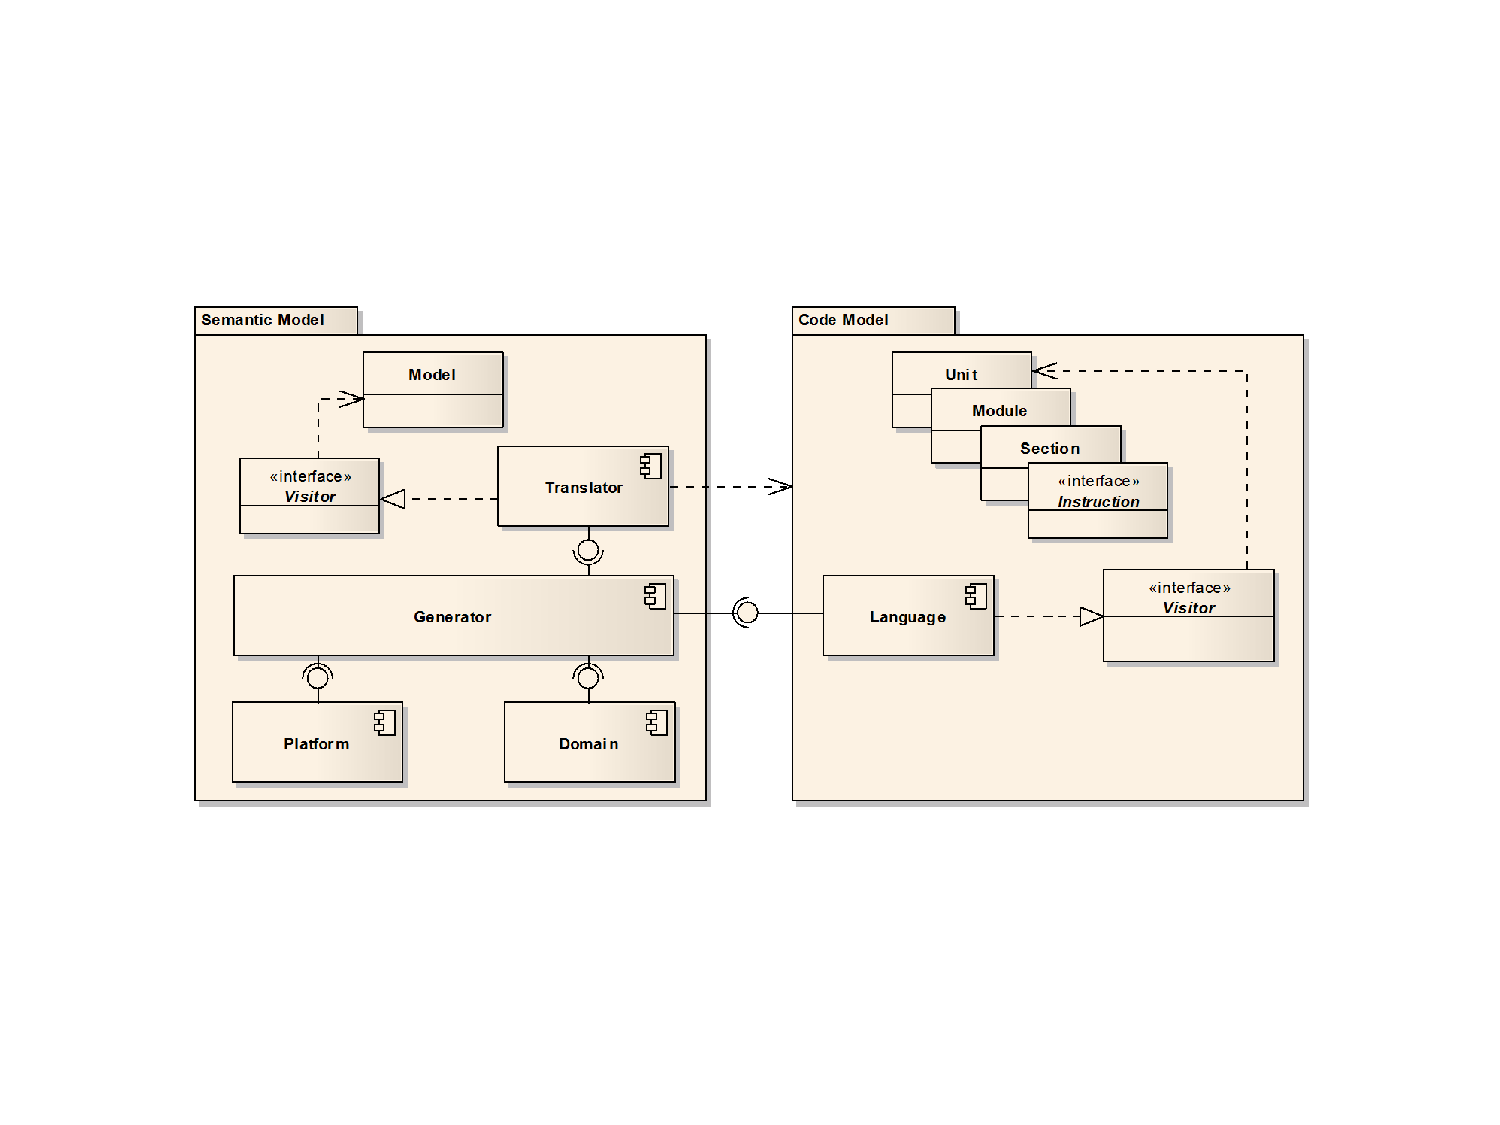
\includegraphics[width=\linewidth]{resources/component-overview.pdf}
  \caption{Overzicht van componenten en kernentiteiten}
  \label{fig:devel-component-overview}
\end{figure}

\TODO

\subsection{ANTLR}
\label{subsection:devel-antlr}

\TODO

\begin{figure}[ht]
  \centering
  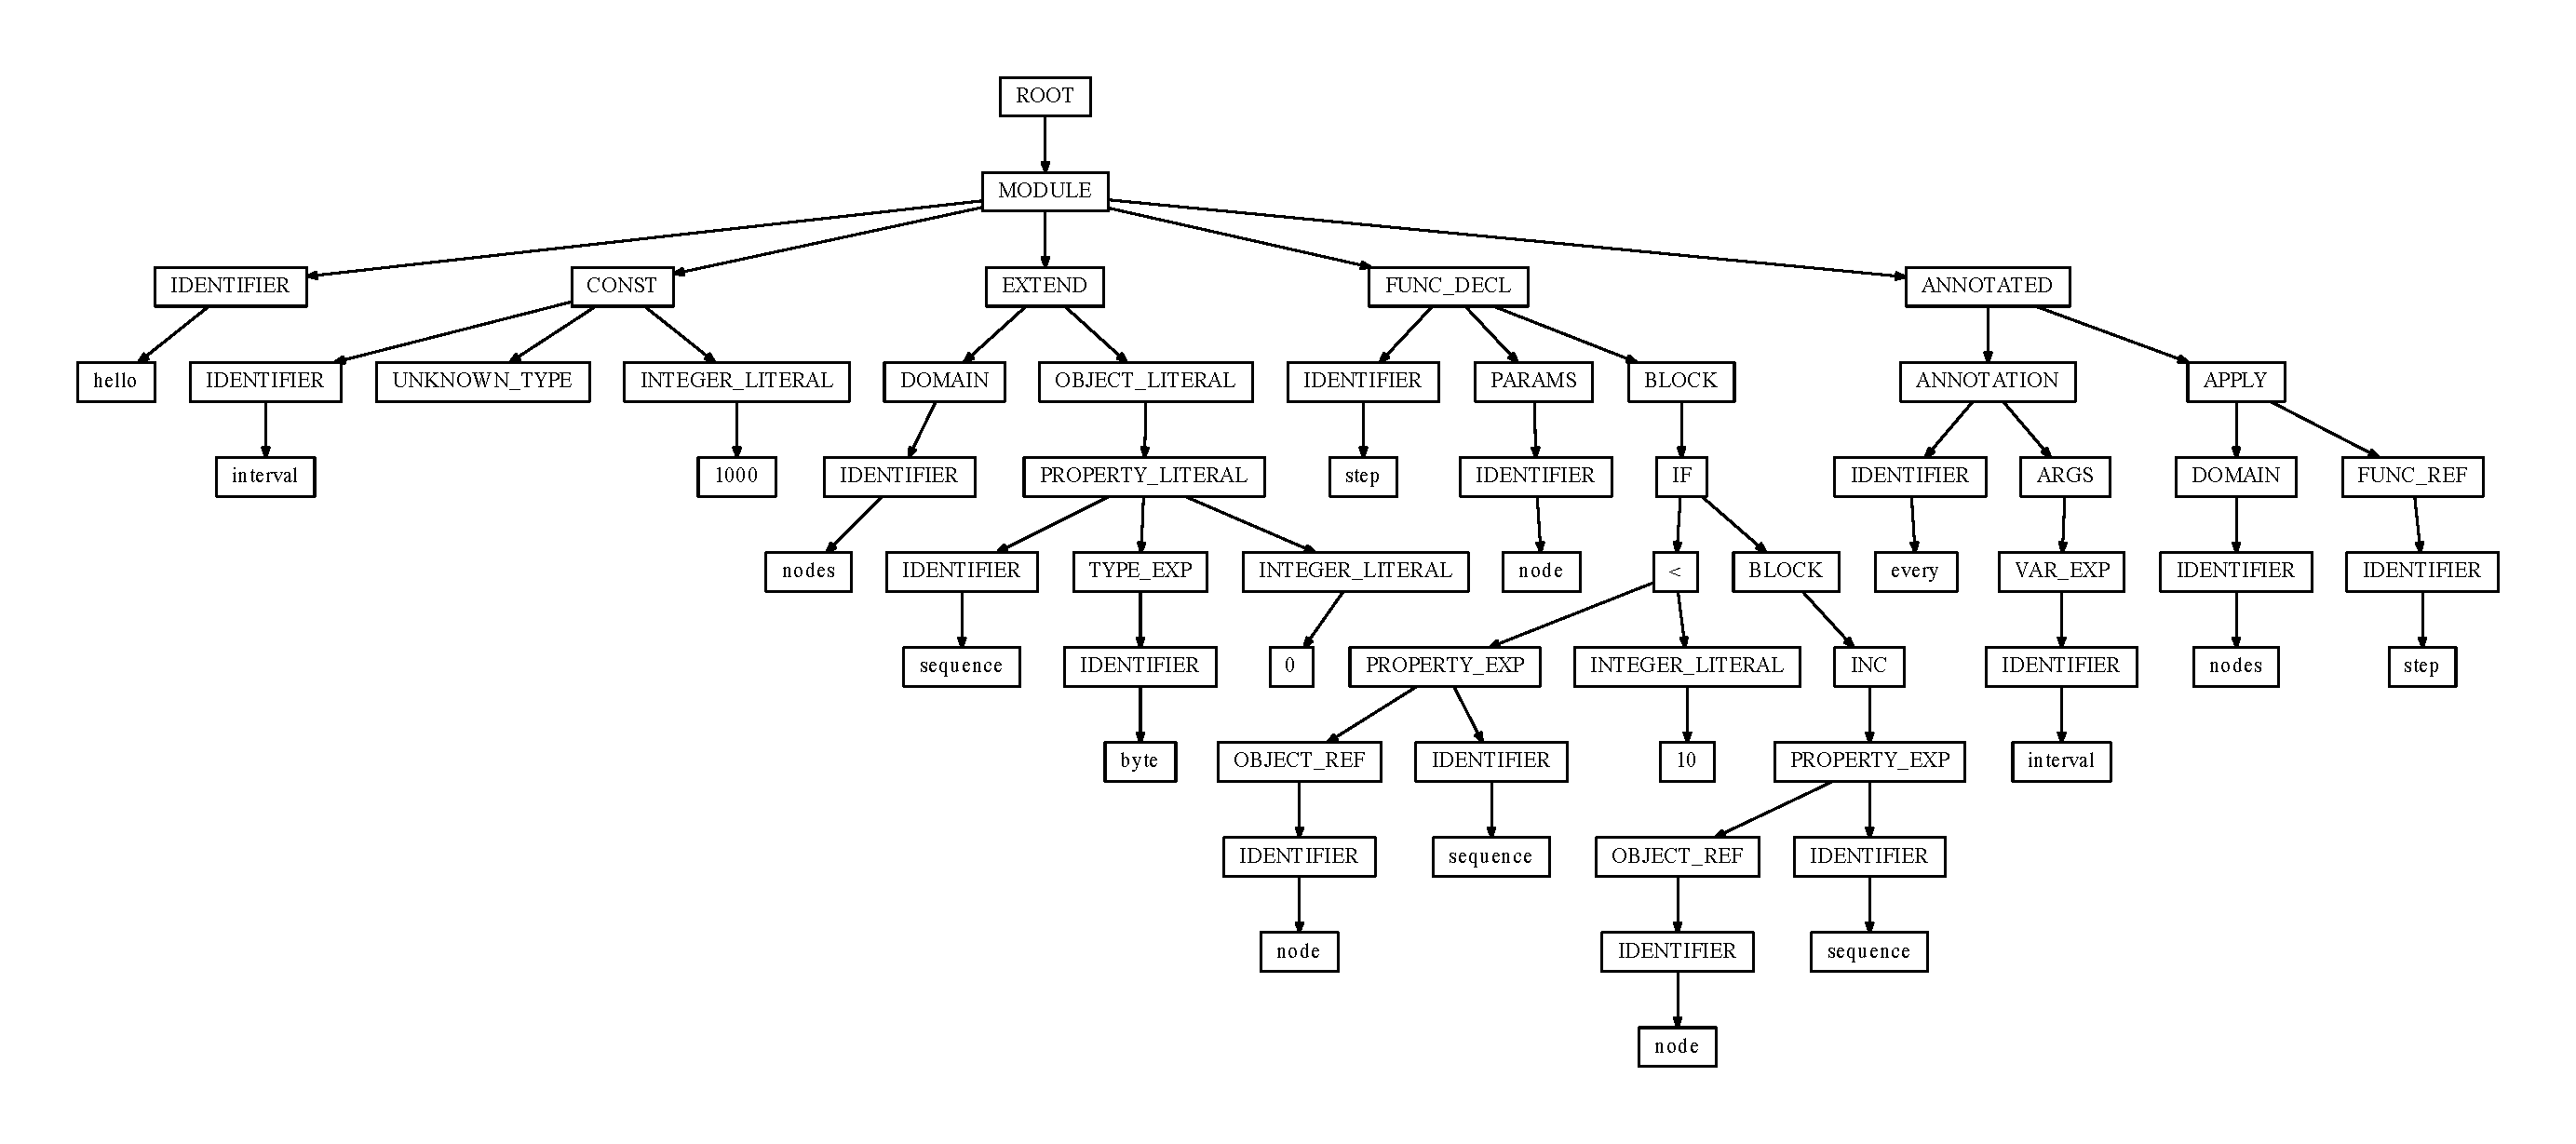
\includegraphics[width=\linewidth]{resources/hello_ast.pdf}
  \caption{Een AST}
  \label{fig:devel-ast}
\end{figure}

\TODO

\subsection{Interfaces}
\label{subsection:devel-codegen-interfaces}

\TODO

- api
- foo

\subsection{Semantisch model}
\label{subsection:devel-semantic-model}

\TODO

- inferrer
- checker

\subsection{Code model}
\label{subsection:devel-code-model}

\TODO

\subsection{Transformaties}
\label{subsection:transformations}

\TODO

\subsubsection{Het visitor patroon}
\label{subsubsection:devel-visitor-pattern}

\TODO

\section{FOO-lib}
\label{section:devel-foo-lib}

\TODO
